\section{Trial Wave Function}
An accurate trial wave function can drastically improve the accuracy of a variational QMC method such as VMC. Most highly accurate trial wave functions are entirely computationally intractable and are never implemented in QMC methods. In addition to being accurate and computationally tractable we seek for wave functions that satisfy known physical properties such as cluster decomposition as well as having an overall antisymmetry with respect to particle exchange due to nucleons obeying fermi statistics.

Cluster decomposition arises from the physical intuition that the wave function of two separate, non-interacting systems, $A$ and $B$ as in Figure~\ref{fig:cluster}, can be written as the product of their respective wave functions.
\begin{figure}[h]
   \centering
   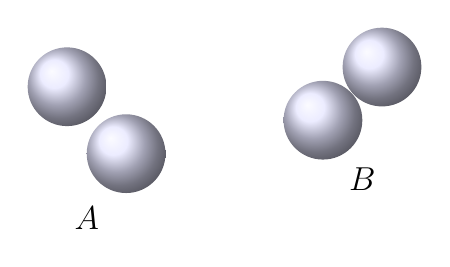
\begin{tikzpicture}[>=latex,scale=0.5]
      \shade[ball color=blue!10!] (-4.0,0.85) circle (1) ;
      \shade[ball color=blue!10!] (-2.5,-0.85) circle (1) ;
      \shade[ball color=blue!10!] (4.0,1.35) circle (1) ;
      \shade[ball color=blue!10!] (2.5,0.00) circle (1) ;
      \draw (-3.5,-2.5) node{\large $\ket{A}$};
      \draw (3.5,-1.5) node{\large $\ket{B}$};
   \end{tikzpicture}
   \caption{Two non interacting systems $A$ and $B$, whose composite wave function is the product $\ket{A+B}=\ket{A}\ket{B}$.}
   \label{fig:cluster}
\end{figure}
Mathematically this can be represented as a product of $n$-body functions, where $n$ is often 1 or 2 in our situation, though it could be higher. If a system is not cluster decomposable then unphysical correlations between non-interacting systems can occur.

The second property is that the wave function be antisymmetric overall. Since nucleons are fermions and the only degrees of freedom used in these calculations the product of different pieces of the wave function must be antisymmetric. Recent work in QMC has successfully included bosonic degrees of freedom such as pions \cite{madeira2018}, however that is not the case in this work.

%\begin{figure}[h!]
%   \centering
%   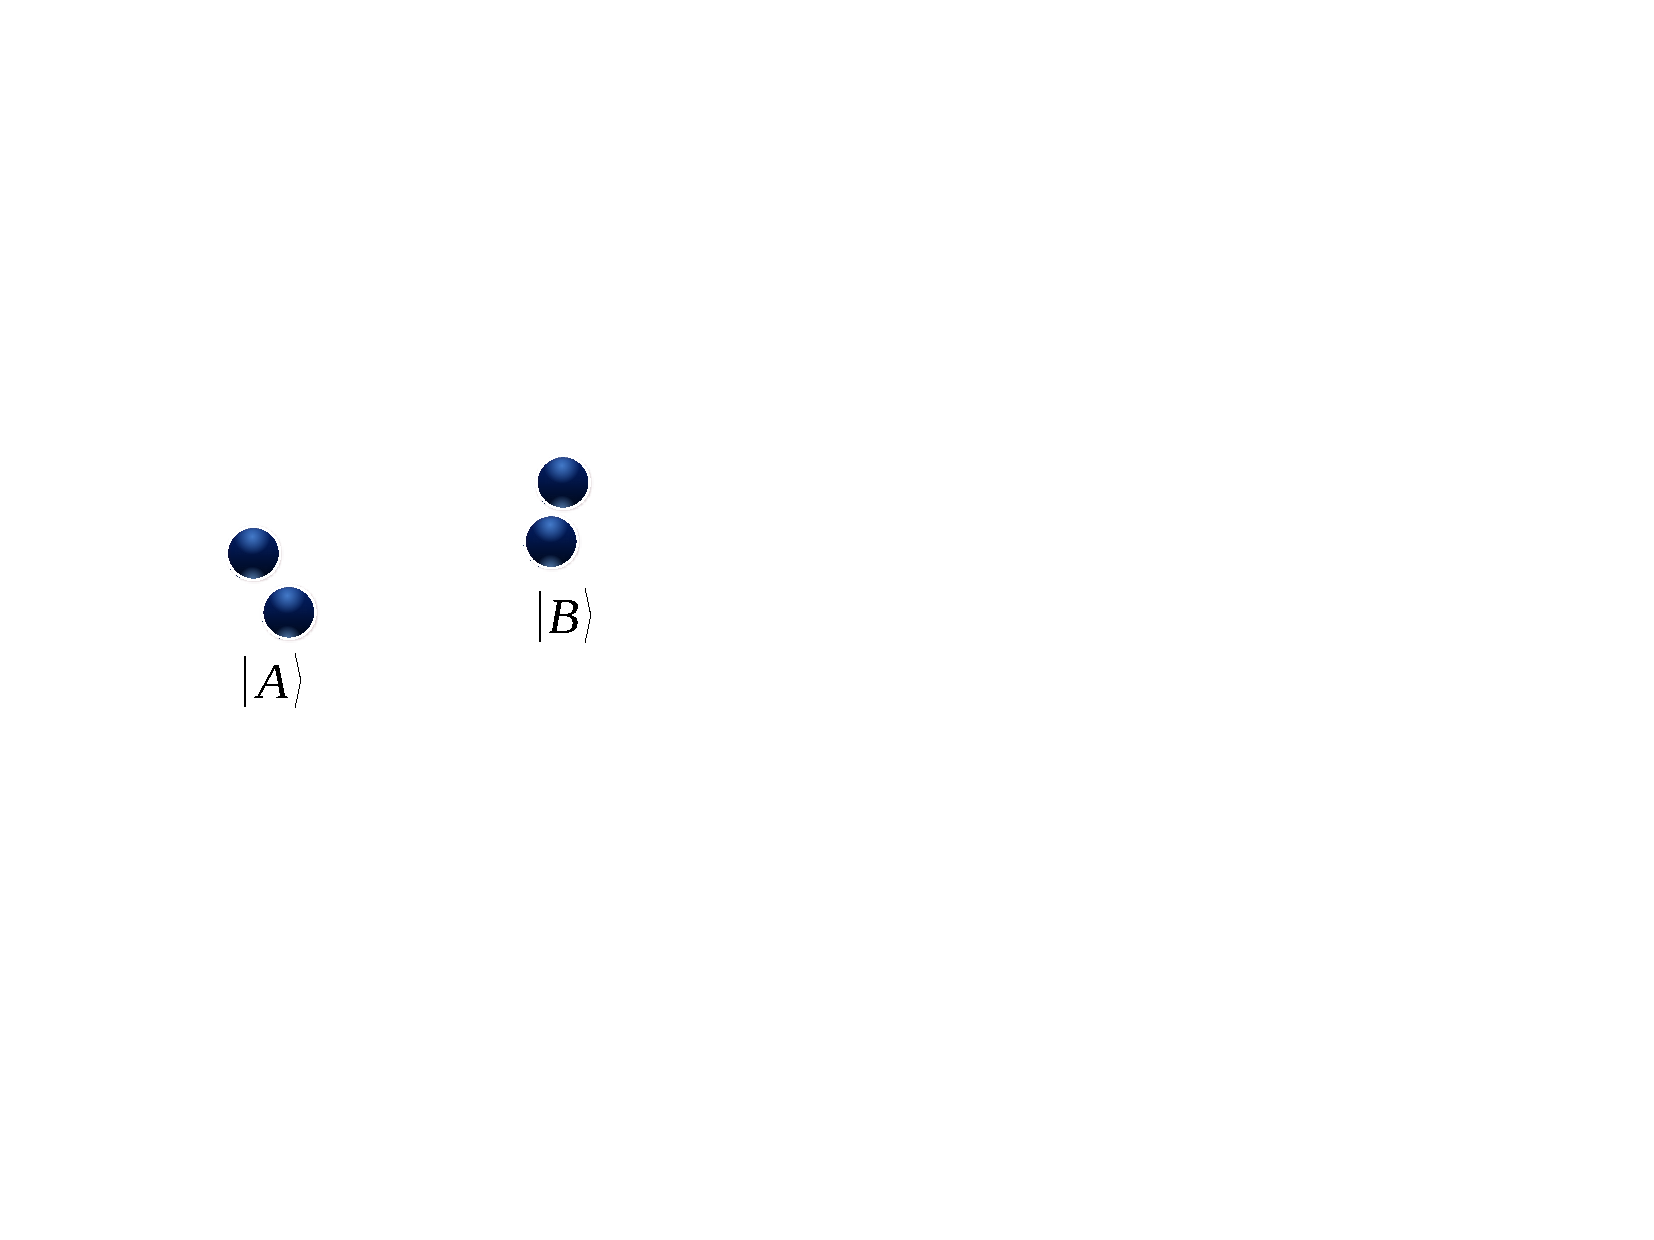
\includegraphics[width=\textwidth]{figures/cluster.pdf}
%   \caption{Energy per nucleon for ${}^4$He and ${}^{16}$O as calculated with linear, independent pair and quadratic correlations. Also, the energy per nucleon of symmetric nuclear matter of 28 particles in a periodic box with density $\rho=0.16$fm$^{-3}$. All calculations are compared to their expected values.}
%   \label{fig:cluster}
%\end{figure}

\subsection{Slater Determinant}
One of the simplest wave functions that satisfies the two properties specified above is the Slater determinant. The Slater determinant has been the starting place for a variety of many-body calculations in nuclear and condensed matter physics alike. In condensed matter the many-body wave functions will often be written in terms of a sum of weighted Slater determinants, where some methods have been able to use a sum of up to 2 billion determinants \cite{huron1973,li2018}. In nuclear physics we often use a single determinant for closed shell calculations and sum of a small number, $\mathcal{O}(10)$, of weighted determinants for open shell systems. A Slater determinant is an antisymmetrized product of single particle (non-interacting) wave functions
\begin{equation}
   \Psi_{SD} = \mathcal{A} \left[\phi_1(\r_1)\phi_2(\r_2) \ldots \phi_A(\r_A)\right] =
   \begin{vmatrix}
      \phi_1(\r_1) & \phi_1(\r_2) & \ldots & \phi_1(\r_A) \\
      \phi_2(\r_1) & \phi_2(\r_2) & \ldots & \phi_2(\r_A) \\
      \vdots & \vdots & \ddots & \vdots \\
      \phi_K(\r_1) & \phi_K(\r_2) & \ldots & \phi_K(\r_A) \\
   \end{vmatrix},
\end{equation}
where the $\mathcal{A}$ is the antisymitrization operator and the $\phi_i(\r_j)$ are the overlap with the walker positions and the model single particle states. In practice the
\red{Make sure to include Jastrow Correlations}

\subsection{Pfaffian Wave Function}

\subsection{Spin-Isospin Dependent Correlations}
\red{Explain what properties you need, etc.}

\subsubsection{Quadratic Correlations}
\red{Be sure to include results}

\subsubsection{Exponential Correlations}
\red{Why aren't they working}

\subsubsection{Alessandro's correlations and $T^2$ fix to them - \red{Maybe just do $T^2$ fix and apply it to exponential correlations}}
